\documentclass[xcolor=table]{article}
\usepackage{DejaVuSansMono}
\usepackage{ragged2e}
\usepackage{pstricks}
\usepackage{pst-eps}
\usepackage{pst-node}
\usepackage{savesym}
\usepackage{pifont}
\usepackage{graphicx}
\begin{document}
\TeXtoEPS
\fontfamily{DejaVuSansMono-TLF}\selectfont
\begin{pspicture}(0,0)(20,6.5)
\newrgbcolor{funkybackground}{0.5 0.6 0.7}
\rput[bl](0,0){\pspolygon*[linecolor=funkybackground,linewidth=0pt](0,0)(30,0)(30,8)(0,8)(0,0)}
\rput[bl](2,0){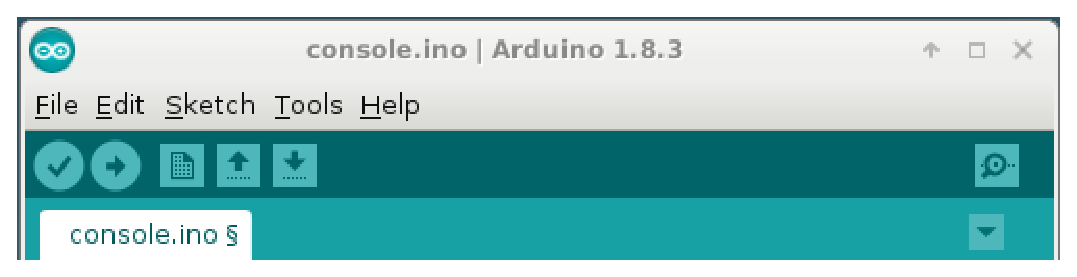
\includegraphics{opensc-input.eps}}
%\rput[bl](0,0){\psgrid(0,0)(30,8)}
\fontsize{24}{24}\selectfont
\rput[bl](0.5,5){\textcolor{blue}{Click here to open the Serial Console}}
\pnode(4.2,5){A}
\cnode[linewidth=5pt,linecolor=yellow](18.5,1.6){1}{B}
%	\nccurve[angleA=-90,angleB=90,arrowsize=10pt]{->}{A}{B}
\ncline[linecolor=red,linewidth=4pt,arrowsize=12pt]{->}{A}{B}
\end{pspicture}
\endTeXtoEPS
\end{document}
